\chapter{Snake Game}

A snake game is an arcade maze game which has been developed by Gremlin Industries and published by Sega in October 1976. It is considered to be a skillful game and has been popularized among people for generations. The snake in the Snake game is controlled using the four direction buttons relative to the direction it is headed in. The player’s objective in the game is to achieve as many points as possible by collecting food or fruits. The player loses once the snake hits the wall or hits itself.

So, we will be creating a Python-based game using the following modules:

\begin{enumerate}
  \item \textbf{Turtle}: It is a pre-installed Python library that enables users to create shapes and pictures by providing them with a virtual canvas.
  \item \textbf{Time}: This function is used to count the number of seconds elapsed since the start.
  \item \textbf{Random}: This function is used to generate random numbers in Python by using a random module.
\end{enumerate}

\section{Steps to Implement Snake Game using Turtle in Python}

\begin{figure}[t]
\centering
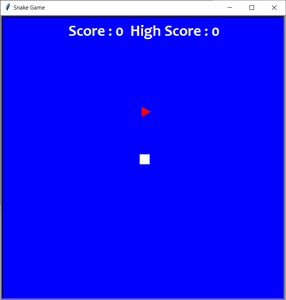
\includegraphics[width=0.6\textwidth]{PART3/2_snake_game/image.png}
\caption{Snake Game GUI}
\end{figure}

\subsection{Step 0: Make a New Python Scripts}
Make a new script and name it \texttt{snake.py}.

\subsection{Step 1: Prepare The Environment}

\begin{enumerate}
    \item \textbf{Import Modules}: The turtle, time, and random modules are imported for creating the snake game, controlling time delays, and generating random values for the food.
\begin{lstlisting}[language=Python]
import turtle
import time
import random
\end{lstlisting}
  
  \item \textbf{Game Settings}: Variables for delay, score, and high score are initialized.
\begin{lstlisting}[language=Python]
delay = 0.1 # seconds
score = 0
high_score = 0
\end{lstlisting}
  
  \item \textbf{Window Setup}: A window is created with a title, blue background, and a size of 600×600 pixels.
\begin{lstlisting}[language=Python]
wn = turtle.Screen()
wn.title("Snake Game")
wn.bgcolor("blue")
% the width and height can be put as user's choice
wn.setup(width=600, height=600)
wn.tracer(0)
\end{lstlisting}

  \item \textbf{Snake Head}: A turtle object is created to represent the snake’s head, with an initial position at the center (0, 0) and its movement direction set to “Stop”.
\begin{lstlisting}[language=Python]
head = turtle.Turtle()
head.shape("square")
head.color("white")
head.penup()
head.goto(0, 0)
head.direction = "Stop"
\end{lstlisting}

\clearpage
\item \textbf{Food Setup}: Another turtle object is created to represent the food, with a random color and shape, positioned at (0, 100).
\begin{lstlisting}[language=Python]
food = turtle.Turtle()
colors = random.choice(['red', 'green', 'black'])
shapes = random.choice(['square', 'triangle', 'circle'])
food.speed(0)
food.shape(shapes)
food.color(colors)
food.penup()
food.goto(0, 100)
\end{lstlisting}

  \item \textbf{Score Display}: A hidden turtle object is used to display the score and high score on the screen, starting with “Score: 0 High Score: 0” in the center of the window.
\begin{lstlisting}[language=Python]
pen = turtle.Turtle()
pen.speed(0)
pen.shape("square")
pen.color("white")
pen.penup()
pen.hideturtle()
pen.goto(0, 250)
pen.write("Score : 0  High Score : 0", align="center",
          font=("candara", 24, "bold"))
\end{lstlisting}
\end{enumerate}

\subsection{Step 2: Set-up Game Controls}

This code defines a simple snake movement mechanism, likely for a game. Each function handles a key direction:

\begin{enumerate}
  \item \texttt{goup()} sets the snake’s direction to “up” unless it’s currently moving “down.”
\begin{lstlisting}[language=Python]
def goup():
    if head.direction != "down":
        head.direction = "up"
\end{lstlisting}

  \item \texttt{godown()} sets the direction to “down” unless moving “up.”
\begin{lstlisting}[language=Python]
def godown():
    if head.direction != "up":
        head.direction = "down"
\end{lstlisting}

  \item \texttt{goleft()} sets the direction to “left” unless moving “right.”
\begin{lstlisting}[language=Python]
def goleft():
    if head.direction != "right":
        head.direction = "left"
\end{lstlisting}

  \item \texttt{goright()} sets the direction to “right” unless moving “left.”
\begin{lstlisting}[language=Python]
def goright():
    if head.direction != "left":
        head.direction = "right"
\end{lstlisting}

\item \texttt{move()} checks the snake’s current direction and updates its position by adjusting its x or y coordinates.
\begin{lstlisting}[language=Python]
def move():
    if head.direction == "up":
        y = head.ycor()
        head.sety(y+20)
    if head.direction == "down":
        y = head.ycor()
        head.sety(y-20)
    if head.direction == "left":
        x = head.xcor()
        head.setx(x-20)
    if head.direction == "right":
        x = head.xcor()
        head.setx(x+20)
\end{lstlisting}

Additionally, keyboard listeners (\texttt{wn.onkeypress}) are set up to control the snake’s direction when the keys \texttt{w}, \texttt{s}, \texttt{a}, or \texttt{d} are pressed, corresponding to up, down, left, and right movements. The snake segments are stored in the segments list.

\begin{lstlisting}[language=Python]
wn.listen()
wn.onkeypress(goup, "w")
wn.onkeypress(godown, "s")
wn.onkeypress(goleft, "a")
wn.onkeypress(goright, "d")

segments = []
\end{lstlisting}
\end{enumerate}

\subsection{Step 3: Set-up Game Loop}

This code is part of a game implemented using the Python turtle module, likely a variant of the classic “Snake” game. Here’s a breakdown of its functionality:

\begin{enumerate}
  \item \textbf{Main Game Loop}: The \texttt{while True} loop continuously updates the game window to keep the game running. The loop only ends when the game is manually stopped or interrupted.
\begin{lstlisting}[language=Python]
# Main Gameplay
while True:
    # Logic here
\end{lstlisting}

\clearpage
\item \textbf{Boundary Collision Check}: The game checks if the snake’s head (head) has moved outside the predefined game area boundaries (\texttt{xcor()} \textgreater 290 or \textless -290, or \texttt{ycor()} \textgreater 290 or \textless -290). If so, the snake is reset to the center of the screen, and all segments of the snake are moved off-screen (to coordinates 1000, 1000), effectively resetting the snake’s length. The score is also reset to zero, and the game speed (delay) is reset.
\begin{lstlisting}[language=Python]
    if head.xcor() > 290 or head.xcor() < -290 or head.ycor() > 290  or head.ycor() < -290:
        time.sleep(1)
        head.goto(0, 0)
        head.direction = "up"
        colors = random.choice(['red', 'blue', 'green'])
        shapes = random.choice(['square', 'circle'])
        for segment in segments:
            segment.goto(1000, 1000)
        segments.clear()
        score = 0
        delay = 0.1
        pen.clear()
        pen.write("Score : {} High Score : {} ".format(score,high_score), align="center", font=("candara", 24, "bold"))
\end{lstlisting}

\item \textbf{Food Interaction}: If the distance between the snake’s head and the food is less than 20 units, indicating a collision, the food is relocated to a new random position within game boundaries. A new segment is added to the snake to increase its length, the game’s delay decreases slightly to increase speed, and the score increases by 10 points.
\begin{lstlisting}[language=Python]
    if head.distance(food) < 20:
        x = random.randint(-270, 270)
        y = random.randint(-270, 270)
        food.goto(x, y)

        % Adding segment
        new_segment = turtle.Turtle()
        new_segment.speed(0)
        new_segment.shape("square")
        new_segment.color("orange")  % tail colour
        new_segment.penup()
        segments.append(new_segment)
        delay -= 0.001
        score += 10
        if score > high_score:
            high_score = score
        pen.clear()
        pen.write("Score : {} High Score : {} ".format(
            score, high_score), align="center", font=("candara", 24, "bold"))
\end{lstlisting}

\item \textbf{Segment Movement Logic}: Each segment of the snake follows the one in front of it, creating a trailing effect. This is done by moving each segment to the position of the segment in front of it, starting from the last segment and moving backwards through the list.
\begin{lstlisting}[language=Python]
    for index in range(len(segments)-1, 0, -1):
        x = segments[index-1].xcor()
        y = segments[index-1].ycor()
        segments[index].goto(x, y)
    if len(segments) > 0:
        x = head.xcor()
        y = head.ycor()
        segments[0].goto(x, y)
    move()  % moves the head
\end{lstlisting}

\item \textbf{Head-Segment Collision}: The game checks for collisions between the snake’s head and its body segments. If such a collision occurs (distance < 20), the snake is reset to the center, similar to the boundary collision behavior, and the game state is reset as described earlier.
\begin{lstlisting}[language=Python]
    for segment in segments:
        if segment.distance(head) < 20:
            time.sleep(1)
            head.goto(0, 0)
            head.direction = "up"
            colors = random.choice(['red', 'blue', 'green'])
            shapes = random.choice(['square', 'circle'])
            for segment in segments:
                segment.goto(1000, 1000)
            segments.clear()

            score = 0
            delay = 0.1
            pen.clear()
            pen.write("Score : {} High Score : {} ".format(
                score, high_score), align="center", font=("candara", 24, "bold"))
\end{lstlisting}

  \item \textbf{Delay Management}: The game’s responsiveness or speed is controlled by \texttt{time.sleep(delay)}, which pauses the game loop to slow down the snake’s movement, making the game manageable.
\begin{lstlisting}[language=Python]
    time.sleep(delay)
\end{lstlisting}
\end{enumerate}

\section{Run the Script}

Run the script using the Run button, or write the following command in your terminal:
\begin{lstlisting}[language=bash]
python snake.py
\end{lstlisting}